%!TEX root = ../doc.tex
\chapter{Implementation}
\label{sec:Implementation}
This chapter describes the implementation and the connections of the individual components of the augmented reality system. There are two main tasks, the system needs to perform: A three dimensional estimation of the surrounding and the precise measurement of motion of the camera head.
\section{Hardware}
\label{sec:Hardware}
The following section describes the evaluation and setup of the hardware used for the camera head and the processing system. 
\subsection{Evaluation of ToF Camera}
\label{sec:CamEvaluation}
Having no prior experience with time-of-flight (ToF) cameras, a suitable device had to be evaluated first. Cost and availability have been the main factors in the evaluation, with it being directly CSI-2 connected being a big plus.\\
Internet research has shown a handful of different sensors powering multiple products of other manufacturers in varying price ranges. \\
\\
\textbf{Sony DepthSense IMX556PLR}\\
The Sony IMX556PLR ToF Sensor offers a resolution of 640 x 480 pixels at 30 frames per second and is used by Basler, Lucid Vision Labs, and DephtEye, primarily for Gigabit Ethernet cameras. The IMX556PLR seems to be the most capable ToF sensor freely available in off-the-shelf products at the time.  \\
The technically most compelling product for this thesis would have been the Helios Flex by Lucid Vision Labs, which directly connects via CSI-2 and is sold specifically for use on an Nvidia Jetson TX2 Developer Kit. It features a maximum range of 6 meters for depth measurement and accuracy of ±10mm. Although with 749 US Dollars, the Helios Flex is relatively expensive and unsuitable for the thesis because of an unknown lead time.\\
\\
\textbf{Infineon REAL3 IRS1125}\\
The Infineon IRS1125 ToF Sensor is available in a USB-based development kit by pmdtec – an integrator for ToF technology into smartphones – and on the affordable PiEye Nimbus 3D camera, which is sold as a Raspberry Pi accessory.  \\
The sensor features a resolution of 352x288 pixels at 30 frames per second in the variant IRS1125A. The variant IRS1125C – used by pmdtec – allows 60 frames per second. The pmdtec development kit is tuned for measuring up to 6 meters, while the PiEye camera is limited to 5 meters.\\
While both camera systems are readily available to be shipped, the pmdtec pico monstar costs about 1500 US Dollars; in contrast, the PiEye Nimbus costs only 230 Euros. The PiEye company advertises its camera with open source software to embed it into the Raspberry Pi ecosystem. However, further investigation has shown that the middleware – the library managing the camera’s settings and connecting to the video4linux2 framework – is still under NDA with Infineon. \\
With a lightweight TCP/IP protocol, the module is suitable with a Raspberry Pi, acting as a Gigabit Ethernet camera. The PiEye Nimbus is the module of choice for this thesis – the availability, the price, and the specifications are all reasonable. The options to reverse engineer the middleware or sign an individual NDA with Infineon have been kept open initially but were not necessary as the Gigabit Ethernet implementation worked well enough.\\
\\
\textbf{Other image sensors}\\
During the internet research, the Texas Instruments OPT8241 has shown up. TI declared the chip obsolete – the chip itself was still available, but the development kit was sold out. With 320 times 240 pixels and an advertised range of 4 meters, the OPT8241 is inferior to the chosen PiEye Nimbus. In addition, the Terabee 3Dcam features a custom sensor with a resolution of 80x60 pixels and 4 meters range. It is attached by USB 2.0 and costs 250 Euros. Due to the low resolution, the Terabee 3Dcam is also inferior to the PiEye Nimbus. 


\subsection{Camera Head}
\label{sec:camHead}
The camera head contains the PiEye Nimbus ToF camera, mounted on a Raspberry Pi 4B, a Bosch BMI160 IMU, attached to a USB to I²C bridge, and a standard Raspberry Pi camera v2.1 which is connected to the processing system via an FPDLink module.\\
All is held together by a plywood structure glued onto a tripod-baseplate, shown in figure \ref{fig:cameraHead}.
\begin{figure}[H]
    \centering
    \begin{minipage}[b]{0.45\textwidth}
      
\includegraphics[scale=0.40]{images/todo.png}
      \caption{Frontside}
      \label{fig:cameraHeadfront} 
    \end{minipage} % Hier darf keine Leerzeile zwischen den beiden Minipages liegen!
    \begin{minipage}[b]{0.45\textwidth}
      
\includegraphics[scale=0.40]{images/todo.png} 
      \caption{Backside}
      \label{fig:cameraHeadback} 
    \end{minipage}
    \caption{The camera head consisting of the ToF camera, the IMU and the Raspberry Pi camera}
    \label{fig:cameraHead}
  \end{figure}
The IMU could have been attached directly to the Raspberry Pi, but at the time of the implementation, the decision on how to connect the ToF camera was not taken yet. Therefore, it was not certain that a Raspberry Pi would be mounted at the camera head.
Four individual cables connect to the different components on the camera head: A USB-C power cable and an RJ45 Ethernet cable for the Raspberry Pi, a USB 2.0 cable for the USB to I²C bridge, and an FPDLink coaxial cable for the Raspberry Pi Camera.


\subsection{Processing System}
\label{sec:procSystem}
An Nvidia Jetson Xavier AGX in the 8GB version carries out the processing, rendering, and data acquisition. An Anyvision baseboard - shown in image \ref{fig:anyvision} - carries the Nvidia Jetson module and allows the direct attachment of the used data cables.
\begin{figure}[H]
    \centering
    
\includegraphics[width=1.0\textwidth]{images/todo.png}
    \caption{The Nvidia Jetson Xavier AGX on the Anyvision Baseboard.}
    \label{fig:anyvision}
\end{figure}
A TCP/IP server application on the Raspberry Pi powering the PiEye ToF camera, to which the processing system connects, serves the necessary ToF camera data in a frame-based protocol. The USB to I²C bridge gets loaded as a standard I²C device by the Linux on the processing system. The IMU is then directly configured and polled by the userspace software on the processing system without an additional driver. The Raspberry Pi camera is attached via FPDLink and integrated as a video4linux2 device. The capturing is done with FFMPEG and the debayering in CUDA.
\section{Video inputs}
\label{sec:videoInputs}
The system utilizes two cameras, a Raspberry Pi Camera v2 and a PiEye ToF camera that doubles as an infrared camera. The Sony IMX 219 based Raspberry Pi Camera v2 features a color image with an 8 megapixel resolution for single images, 1080p with 30 frames per second, 720p with 60 frames per second or 480p with 90 frames per second.\cite{raspiCamSpec} The Raspberry Pi Camera v2 is a Mipi CSI2 attached camera module whichs cable length got extended by an FPDLink serializer and deserializer.\\
The PiEye ToF camera is based on the Infineon REAL3 IRS1125A sensor which has a resolution of 352 x 288 pixels\cite{piEyeShop}. The ToF Camera is paired with infrared LED flashes to measure the time of flight of the light emitted and has an intended measurement range from 10 centimeters up to five meters. The entire ToF software stack runs on a Raspberry Pi that sends its video data via Ethernet to the augmented reality system.\\

\subsection{ToF Camera calibration}
\label{sec:ToFCalibration}
On the ToF Camera, two parts need to be calibrated: The optics, as described in section \ref{sec:FundCamCalibration}, and the distance measurement. The ToF camera has a barrel type distortion that is corrected by the camera calibration algorithm implemented in OpenCV\cite{openCVCamCalib} and shown in image \ref{fig.camCalib}. As the process of lens correction cuts off parts of the image, the image size gets lowered to 265 x 205 pixels.\\
For the distance measurement, first the radial distances need to be flattened as described in section \ref{sec:RadialCorrection}. As the angle $\alpha$ is not known for each pixel, a reference measurement provides the necessary information. To reduce noise, 19 images of the same flat wall has been taken, smoothed by a gaussian and averaged onto one reference image $I_{Ref}$. The wireframe image in figure \ref{im:ToFRaw} shows the curvature of the reference image. The rounding at the edges is an arfifact of the gaussian smoothing.\\
\begin{figure}[H]
    \centering
    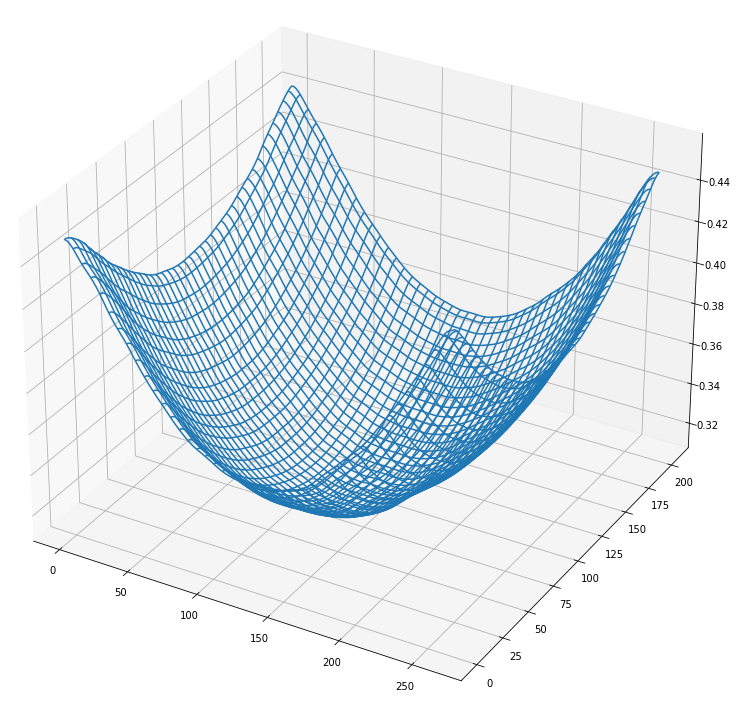
\includegraphics[width=0.4\textwidth]{images/raw_tof_radial.png}
    \caption{Wireframe rendering of the reference image $I_{Ref}$ provided by the ToF camera}
    \label{im:ToFRaw}
\end{figure}
Dividing the minimum value of this reference image $I_{Ref}$ with every pixel value generates a map of $\cos \alpha$ named $I_{cos}$.
\begin{equation*}
    I_{cos} = \frac{\min (I_{Ref}) }{I_{Ref}} 
\end{equation*}
Pixel by pixel multiplication of any other image $I_{Any}$ with $I_{cos}$ will correct the influence of the radial measurement as shown in image \ref{im:ToFCorrected}. 
\begin{equation*}
    I_{Corr} = I_{cos}\cdot I_{Any}
\end{equation*}
\begin{figure}[H]
    \centering
    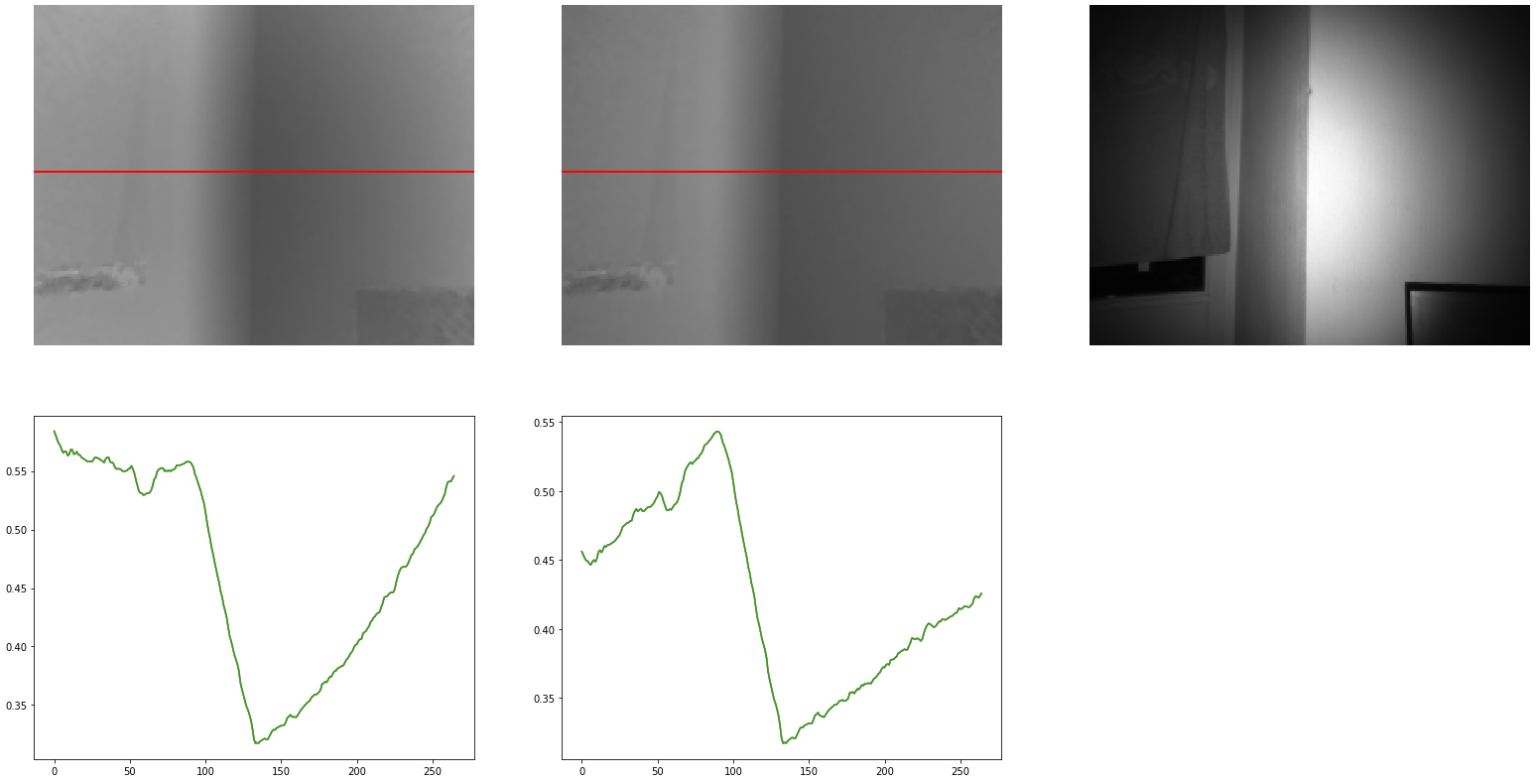
\includegraphics[width=1.0\textwidth]{images/flattened_tof_example.png}
    \caption{Left, the uncorrected ToF image $I_{Any}$, in the middle the corrected image $I_{Corr}$ and on the right, the infrared grayscale image of the scene. To make the effect more apparent, the brightness accross the red lines have been plotted.}
    \label{im:ToFCorrected}
\end{figure}
To apply this calibration in CUDA, a file has been generated which holds the $I_{Cos}$ values for each pixel. The application reads the file at initialization and keeps it stored in a Cuda allocated memory area. 
\subsection{Raspberry Pi Camera calibration}
\label{sec:RBPiCalibration}
The Raspberry Pi camera only provides images for enhancing the system's video output cosmetically; the lens calibration serves no algorithmic purpose. The lens was calibrated solely to map the image into the undistorted Vulkan 3D space, so the virtual rectangle fits the real world's picture.\\
The camera streams in 720p to use the entire sensor with pixel binning. In 1080p, the sensor uses only a portion of the image sensor, which narrows down the field of view. Like with the ToF camera, a lookup table calibrates the Raspberry Pi camera, which reduces the image size to a resolution of 1273 times 709 pixels.

\section{Gyroscope and Accelerometer Calibration}
\label{sec:GyroCal}
The used inertial movement unit (IMU) is a Bosch BMI160, that is sold soldered on a PCB by DFRobot.\\
As the gyroscope and accelerometer output incremental movement, the values need to be integrated over time. Accurate data is crucial for finding the direction of gravity or detecting movement - especially because of positional information being the result of derivating the acceleration twice.\\
The range of the acclerometer is variable and has been set to ±8 G, it has an output resolution of 16 bit and an output data rate of 200 Hz.
The accelerometer has been calibrated in 24 orientations to even out angle errors inside the IMU, on the PCB and of the calibration table, as shown im image \ref{im:IMU_cal}. For each orientation, 100 raw measurements have been averaged to even out noise. 
\begin{figure}[H]
    \centering
    
\includegraphics[width=1.0\textwidth]{images/todo.png}
    \caption{The 24 orientations used for calibration - four directions for each of the six sides.}
    \label{im:IMU_cal}
\end{figure}
The largest error has been 38 mG, that lies within the sensor's specification of ±40 mG\cite{BMI160}. In addition, the gain for the accelerometer has been corrected based on gravity. A maximum error of 1.8\% has been measured and corrected, which also lies in the sensor's specification of ±0.5\% full scale\cite{BMI160}.\\
For the gyroscope, the range is set to ±2000 degrees per second with an output data rate of 200 Hz. The gyroscope has been calibrated only for zero offset, whose maximum error was 0.2 degrees per second which lies well in the specified ±3 degrees per second\cite{BMI160}. A gain correction was not made, because of not having the required equipment to do so.\\
\section{Position and Orientation Estimation}
\label{sec:PositionEstimate}
The position estimation of the camera head is crucial for the augmented reality platform. The following section describes the implementation of the different systems involved in sensing motion.\\
While the measurement using the IMU is standard implementation via I²C communication, the implementation of the ToF-Camera based measurement is more complex and got split into multiple subsections. 
\subsection{Spatial coordinates and device coordinates}
\label{sec:ABC_XYZ_coords}
As the rotation of the camera head changes the coordinates of the measurement in respect to real-world coordinates, a convention helps carry out the calculations. For the sensors on the camera head, the coordinates are named $a$, $b$, and $c$, while the spatial coordinates are named $x$, $y$, and $z$.
The coordinates can be transformed by the following formula, knowing the current orientation quaternion $Q_{rot}$.   
\begin{equation*}
    Q_{rot}
    =
    \begin{pmatrix}
        r           \\
        u\textbf{j} \\
        v\textbf{j} \\
        w\textbf{k}
    \end{pmatrix}
    \quad ; \quad
    \begin{pmatrix}
        0           \\
        x\textbf{i} \\
        y\textbf{j} \\
        z\textbf{k}
    \end{pmatrix}
    =
    \begin{pmatrix}
        r           \\
        u\textbf{i} \\
        v\textbf{j} \\
        w\textbf{k}
    \end{pmatrix}
    \begin{pmatrix}
        0           \\
        a\textbf{i} \\
        b\textbf{j} \\
        c\textbf{k}
    \end{pmatrix}
    \begin{pmatrix}
        r           \\
        -u\textbf{i} \\
        -v\textbf{j} \\
        -w\textbf{k}
    \end{pmatrix}
\end{equation*}
Section \ref{sec:RotationQuaternion} describes how to carry out the mathematics of this quaternion multiplication. 
\subsection{Gyroscope and Accelerometer}
\label{sec:GyroPosition}
The 6-axis IMU Bosch BMI160 provides gyroscope and accelerometer measurements via an I²C connection, extended by a Silicon Labs CP2112 USB-to-I²C bridge. The IMU generates measurements regarding acceleration in the directions $a$, $b$, and $c$, and measurements regarding rotation speed around these axes.\\
The IMU shows a hysteresis that lies within the specification of the datasheet; therefore, a simple offset correction does not yield the best results. A moving average – that gets updated whenever no motion of the camera head is detected – helps deal with the hysteresis by subtraction from the measurement value.
\subsection{ToF Camera: SIFT feature extraction}
\label{sec:ToFPosition_SIFT}
The PiEye Nimbus ToF camera generates three different image channels for each picture taken: The depth map, the confidence, and the greyscale infrared image. By correcting the lens distortion as described in chapter \ref{sec:FundCamCalibration}, straight lines in the real world get projected as straight lines on the images. By further correcting the characteristic of the ToF camera to measure radial distances, as described in section \ref{sec:RadialCorrection}, flat surfaces in the real world are also flat on the depth map. The implementations of both corrections are explained in section \ref{sec:ToFCalibration}. \\
The points of the point clouds need to be matched to estimate rotation and translation between two consecutive ToF images. The CudaSift library\cite{cudaSiftRepo}\cite{CudaSiftPublication} extracts SIFT\cite{siftpaper} features on each greyscale infrared image the ToF camera sends $k$, which are then brute-force matched with the features of the prior image $k-1$, as visualized in image \ref{im:SiftExtraction}. SIFT features were chosen because of the author's prior experience, and it is a well-known feature extraction algorithm whose patent expired.\cite{siftpatent}
\begin{figure}[H]
    \centering
    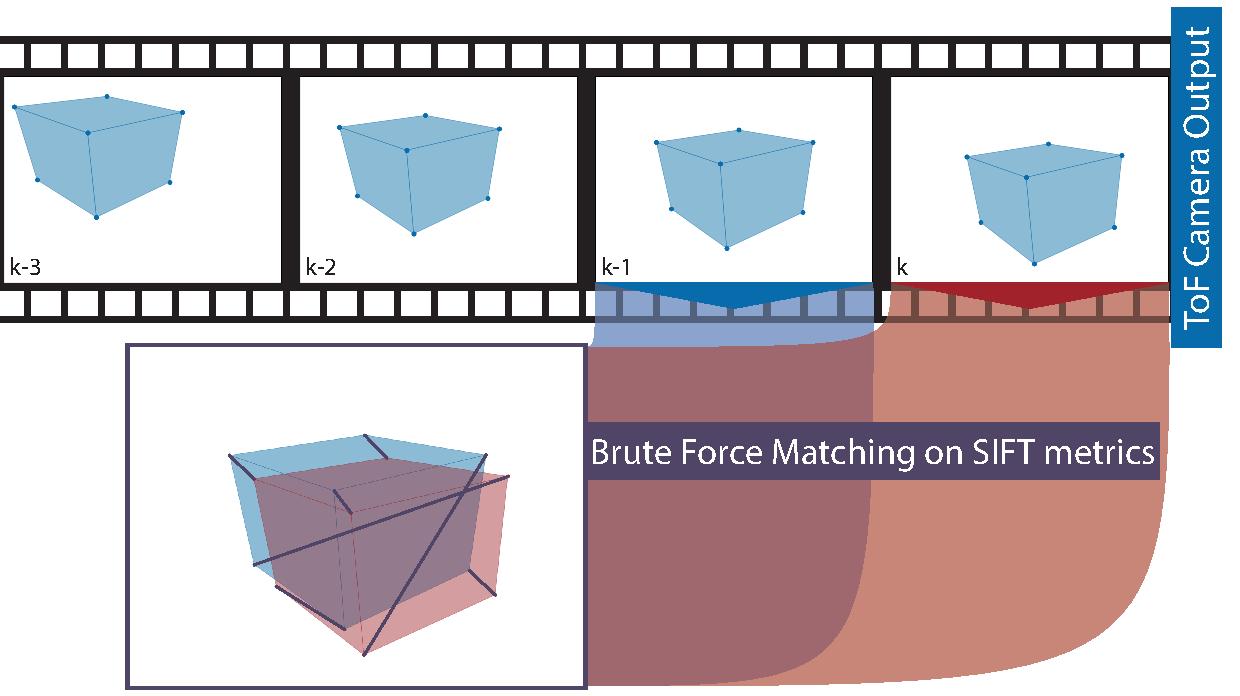
\includegraphics[width=1.0\textwidth]{images/feature_matching_bruteforce.pdf}
    \caption{First step of ToF motion estimation: Extract SIFT features and brute-force match with prior image. Note that the brute-force matcher also generates false matches.}
    \label{im:SiftExtraction}
\end{figure}
Each feature coordinate on the picture gets mapped to the 3D space to generate the point cloud. The lens projects objects within the space of a pyramid onto the sensor, which leads to the following coordinate mapping. The coordinate transformation is visualized in image \ref{im:SiftCoordTransform}. Please note the coordinate convention described in section \ref{sec:ABC_XYZ_coords}. $a$, $b$ and $c$ being the 3D coordinates, $u$ and $v$ being the coordinates on the image and $d$ being the value of the ToF depth image on position $(u,v)$. $f$ denotes a virtual focal length, merging the camera's field of view (viewing angle $\alpha$) and the image resolution in one number.
\begin{equation*}
    a = d \qquad b = \frac{v}{f}\cdot x \qquad c = \frac{u}{f}\cdot x \qquad f=\frac{\tfrac{u_{max}}{2}}{tan(\tfrac{\alpha}{2})}
\end{equation*}
The PiEye Nimbus ToF camera has an advertised viewing angle of $1.152rad$ horizontally and $0.942rad$ vertically. Combined with an image resolution of $352 x 288px$, the formula for $f$ outputs $271$ for the horizontal and $282$ for the vertical case. The chosen value is: $f = 280$.
\begin{figure}[H]
    \centering
    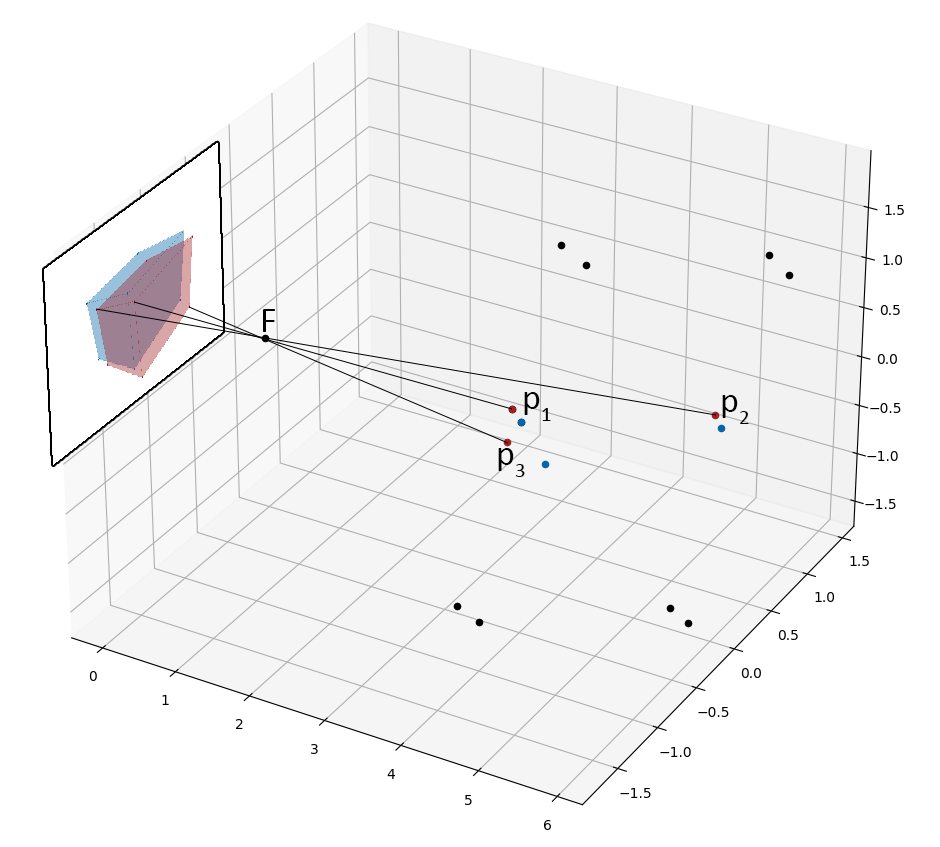
\includegraphics[width=1.0\textwidth]{images/2d_to_3d.png}
    \caption{Second step of ToF motion estimation: Map features into 3D space}
    \label{im:SiftCoordTransform}
\end{figure}
\subsection{ToF Camera: Find rotation and translation}
\label{sec:ToFPosition_SVD}
Calculating the rotation and translation of one point cloud $P_{k-1}$ to another point cloud $P_{k}$ is possible with at least three correctly matched point pairs. Following the recipe from a note from the ETH Zurich, also containing the proof, the three points must be centered. The method described in the ETH note also adds the possibility to add weights to individual data points. Upper case $P$ denotes a point cloud, lower case $p$ denotes a single point in that cloud. The number of matched point pairs in the following formulae is $n$, in the example $n = 3$, $i$ is the index of the single point in the point cloud and $k$ is the image frame number from which the point cloud got extracted.
The centroids for both point groups are:
\begin{equation*}
    \vec{c}_{k}=\frac{\sum_{i=1}^n \vec{p}_{i,k}}{n} \qquad 
    \vec{c}_{k-1}=\frac{\sum_{i=1}^n \vec{p}_{i,k-1}}{n} 
\end{equation*}
For example visualized in image \ref{im:SVD_step_by_step} and with the following calculation:

\begin{equation*}
    \vec{c}_{k}=
    \begin{pmatrix}
        4.421 \\
        -0.154 \\
        0.223
    \end{pmatrix}
    =\frac{1}{3}\cdot\left(
    \begin{pmatrix}
        3.314 \\
        0.043 \\
        -0.037
    \end{pmatrix}
    +
    \begin{pmatrix}
        4.852 \\
        1.198 \\
        -0.586
    \end{pmatrix}
    +
    \begin{pmatrix}
        5.098 \\
        -1.704 \\
        1.291
    \end{pmatrix}
    \right)
\end{equation*}
\begin{equation*}
    \vec{c}_{k-1}=
    \begin{pmatrix}
        4.433 \\
        0.059 \\
        -0.090
    \end{pmatrix}
    =\frac{1}{3}\cdot\left(
        \begin{pmatrix}
            3.298 \\
            0.177 \\
            -0.271
        \end{pmatrix}
        +
        \begin{pmatrix}
            4.709 \\
            1.436 \\
            -0.924
        \end{pmatrix}
        +
        \begin{pmatrix}
            5.291 \\
            -1.436 \\
            0.924
        \end{pmatrix}
    \right)
\end{equation*}
\begin{figure}[H]
    \centering
    
\includegraphics[width=1.0\textwidth]{images/todo.png}
    \caption{Rotation and Translation step by step.}
    \label{im:SVD_step_by_step}
\end{figure}
Subtraction of the centroid vectors from the individual points in the respective point cloud $P$ generates the centered point clouds $Q$. In an ideal case, a rotation matrix alone can transform one centered point cloud into the other. 
\begin{equation*}
    \vec{q}_{i,k}=\vec{p}_{i,k}-\vec{c}_{k} \qquad 
    \vec{q}_{i,k-1}=\vec{p}_{i,k-1}-\vec{c}_{k-1} \qquad i = 1, 2, 3, ... , n
\end{equation*}
In the example, the results are:
\begin{equation*}
    \vec{q}_{1,k}=
    \begin{pmatrix}
        -1.108 \\
        0.197 \\
        -0.260
    \end{pmatrix}
    \qquad 
    \vec{q}_{2,k}=
    \begin{pmatrix}
        0.431 \\
        1.352 \\
        -0.808
    \end{pmatrix}
    \qquad     \vec{q}_{3,k}=
    \begin{pmatrix}
        0.677 \\
        -1.549 \\
        1.068
    \end{pmatrix}
\end{equation*}
\begin{equation*}
    \vec{q}_{1,k-1}=
    \begin{pmatrix}
        -1.134 \\
        0.118 \\
        -0.181
    \end{pmatrix}
    \qquad 
    \vec{q}_{2,k-1}=
    \begin{pmatrix}
        0.276 \\
        1.377 \\
        -0.833
    \end{pmatrix}
    \qquad     \vec{q}_{3,k-1}=
    \begin{pmatrix}
        0.858 \\
        -1.495 \\
        1.014
    \end{pmatrix}
\end{equation*}
A matrix-multiplication of the point groups $Q_{k}$ and $Q_{k-1}$ generates the $3\times3$ covariance matrix $S$ as shown in the following formula. The point groups are packed in matrix form, in the three point example, the point group matrices are of dimension $3\times3$. When using $n$ points, the point group matrices are of dimension $n\times3$, whose covariance matrix remains of dimension $3\times3$.
\begin{equation*}
    S= Q_{k-1}Q_{k}^{T}
\end{equation*}
In the example:
\begin{equation*}
    Q_{k}=
    \begin{bmatrix}
        -1.108 & 0.431  & 0.677  \\
        0.197  & 1.352  & -1.549 \\
        -0.260 & -0.808 & 1.068
    \end{bmatrix} \quad
    Q_{k-1}=
    \begin{bmatrix}
        -1.134 & 0.276  & 0.858  \\
        0.118  & 1.377  & -1.495 \\
        -0.181 & -0.833 & 1.014
    \end{bmatrix}
\end{equation*}
\begin{equation*}
    S= 
    \begin{bmatrix}
        1.956 & -1.180 & 0.989 \\
        -0.549 & 4.201 & -2.741 \\
        0.528 & -2.734 & 1.805
    \end{bmatrix}
\end{equation*}
The singular value decomposition (SVD), briefly explained in section \ref{sec:SVD}, splits the covariance matrix $S$ into three separate $3\times3$ matrices $U$, $\Sigma$, and $V$. As the SVD in this use case is always applied to matrices of dimension $3\times3$, the optimized variant\cite{Gao:2018:GPU_MPM} from GitHub\cite{Github_SVD_CUDA} can be utilized.
\begin{equation*}
    S= U\Sigma V^{T}
\end{equation*}
In the example:
\begin{equation*}
    U=
    \begin{bmatrix}
        -0.301 & -0.950 & -0.080 \\
        0.796 & -0.297 & 0.528 \\
        -0.525 & 0.096 & 0.846
    \end{bmatrix} \quad
    \Sigma=
    \begin{bmatrix}
        6.309 & 0 & 0 \\
        0 & 1.690 & 0 \\
        0 & 0 & 0
    \end{bmatrix} \quad
    V=
    \begin{bmatrix}
        -0.207 & -0.973 & 0.102 \\
        0.814 & -0.229 & -0.534 \\
        -0.543 & 0.028 & -0.839
    \end{bmatrix}
\end{equation*}
The wanted rotation matrix then follows by calculating:
\begin{equation*}
    R=V
    \begin{bmatrix}
        1 & 0 & 0 \\
        0 & 1 & 0 \\
        0 & 0 & det(VU^{T})
    \end{bmatrix}U^{T} \quad
\end{equation*}
Without the correction of the calculation, using the term $det(VU^{T})$ in the intermediate matrix, the method could generate a reflection instead of a rotation. This is numerically sound, but would not reflect the real world scenario. The determinant $det(VU^{T})$ equals -1 in the case of a reflection, which can be used to flip the signs of the 3rd column of the rotation matrix. If the SVD directly generates a rotation, $det(VU^{T})$ equals to 1, which transforms the intermediate matrix into the identity.\\
In the example the resulting rotation matrix $R$ equals:
\begin{equation*}
    R=
    \begin{bmatrix}
        0.995 & 0.071  & -0.071 \\
        -0.071 & 0.998  & 0.002 \\
        0.071& 0.002 & 0.998
    \end{bmatrix} \quad
\end{equation*}
The wanted translation is computed by applying the rotation to the centroid vectors. 
\begin{equation*}
    \vec{t} = \vec{c}_{k}-R\cdot\vec{c}_{k-1}
\end{equation*}
In the example:
\begin{equation*}
    \vec{t} = 
    \begin{pmatrix}
        0 \\
        0.1 \\
        0
    \end{pmatrix}
\end{equation*}
The rotation matrix $R$ and the translation vector $\vec{t}$ fulfill the following equation, in which $p$ are individual points of the point clouds $P$. If the number of points is $n=3$, the calculation is exact, for point clouds with $n>3$ points, the error $E$ is the least-square error\cite{SVD_ETH}.
\begin{equation*}
    \vec{p}_{i,k} = R\cdot\vec{p}_{i,k-1}+\vec{t}+E
\end{equation*}

\subsection{ToF Camera: 3D RANSAC}
\label{sec:ToFPosition_RANSAC}
The motion estimation of the ToF camera relies on having good matches, which is not the case with the brute-force matcher, as the authors of the CudaSift library claim to have less than 50\% accuracy on its brute-force matcher.\cite{cudaSiftRepo} Low matching accuracy is a known problem in other fields of image processing - like panorama stitching - and is there often solved with an algorithm named RANSAC (random sample consensus).\\
These applications of the RANSAC algorithm work on two-dimensional images and are not suitable for three-dimensional point clouds; therefore, the RANSAC algorithm got extended.\\
The first step of the three-dimensional RANSAC is finding a proper rotation and translation from the brute-force matches. To find these transformations, each matched feature pair gets two other feature pairs randomly assigned. Using the method described in section \ref{sec:ToFPosition_SVD}, the corresponding rotations and translations are calculated on these groups of three feature pairs.\\
Each group's calculated rotation matrices and translation vectors get checked against all the other matched feature pairs. The data point from the previous image of the feature pair gets moved by the matrix-vector-pair and compared to the data point of the current picture. If the distance of the two points is underneath a threshold, the feature pair is counted for the matrix-vector-pair. On these feature pairs, the average distance from the calculated points to the matched points is measured. The matrix-vector-pair that generates the smallest average distance is likely suitable for further processing.\\ In a third step, this matrix-vector-pair is recalculated using all brute-force matches within a certain proximity to the calculated point.\\
Ignoring the SIFT metrics that lead to the brute force matching, all the features get matched anew based on the position alone, using the rotation and translation estimated before. The matrix-vector pair transforms every data point from the previous image. The distance between the transformed point and the closest data point of the current picture determines the new match. If the proximity is below a threshold, the match is accepted.\\
Finally, the optimal rotation matrix and translation vector are calculated using the method described in section \ref{sec:ToFPosition_SVD}, this time not with only three points but all accepted matches. With more than three points, the calculated rotation and translation is not the exact result, but the result that yields the least square error.\cite{SVD_ETH}\\
The whole methodology relies on finding the correct rotation and translation from randomly grouped matches. 

\subsection{Sensor Fusion with Kalman Filter}
\label{sec:SensorFusion}
The combination of data coming from different sensors or sensor types is named sensor fusion. In this case, the accelerometer and the calculated motion from the ToF camera add information to the system describing the same movement. Both sensors have noise and inaccuracies that need to be considered to calculate the system state $\vec{x}$, which includes the current position, velocity, acceleration, angular orientation, and angular velocity.\\
A method to estimate the system state is the Kalman filter that allows modeling the system by combining the sensors' uncertainties and the described model itself. The Kalman filter is a discrete predictor-corrector algorithm that uses a system model to predict the next system state using the previous system state $\vec{x}_{k-1}$. The sensor data corrects the system state prediction $\vec{x}_{k|k-1}$ which results in the corrected system state $\vec{x}$.\\
The system requires equal sampling rates for the individual sensors; therefore, the IMU data is downsampled to match the ToF camera's framerate.
With the translational information being present in all three directions and the rotation being inserted in quaternion form, the system state vector $\vec{x}$ has 17 entries. $x$, $y$ and $z$ describe the position in space, and $r_{a}$, $r_{b}$, $r_{c}$, and $r_{d}$ being the components of the orientation quaternion $R = (a, b\textbf{i}, c\textbf{j}, d\textbf{k})$. The time-derivatives of these values are denoted with dots.
\begin{equation*}
    \vec{x}^{T} = (
        x, \dot{x}, \ddot{x}, y, \dot{y}, \ddot{y}, z, \dot{z}, \ddot{z}, r_{a}, r_{b}, r_{c}, r_{d}, \dot{r}_{a}, \dot{r}_{b}, \dot{r}_{c}, \dot{r}_{d})
\end{equation*}
The model $F$ that predicts the intermediate state $\vec{x}_{k|k-1}$ brings the individual entries of the system state into a relationship. The velocities and accelerations both alter the position, while the accelerations alter the velocities. For the rotation, the quaternion containing the angular rotation already contains the sampling rate and gets added by a quaternion multiplication. 
\begin{equation*}
    \vec{x}_{k|k-1} = 
    F
    \cdot
    \vec{x}_{k-1}
\end{equation*}
The $\dot{r}$-values in the matrix are from $\vec{x}_{k-1}$ and $\Delta t$ is the sampling rate.
\begin{equation*}
    \begin{pmatrix}
        x_{k|k-1}\\
        \dot{x}_{k|k-1}\\
        \ddot{x}_{k|k-1}\\
        y_{k|k-1}\\
        \dot{y}_{k|k-1}\\
        \ddot{y}_{k|k-1}\\
        z_{k|k-1}\\
        \dot{z}_{k|k-1}\\
        \ddot{z}_{k|k-1}\\
        r_{a,k|k-1}\\
        r_{b,k|k-1}\\
        r_{c,k|k-1}\\
        r_{d,k|k-1}\\
        \dot{r}_{a,k|k-1}\\
        \dot{r}_{b,k|k-1}\\
        \dot{r}_{c,k|k-1}\\
        \dot{r}_{d,k|k-1}
    \end{pmatrix} = 
    \begin{bmatrix}
        1 & \Delta t & \frac{\Delta t^{2}}{2} & 0 & 0 & 0 & 0 & 0 & 0 & 0 & 0 & 0 & 0 & 0 & 0 & 0 & 0 \\
        0 & 1 & \Delta t & 0 & 0 & 0 & 0 & 0 & 0 & 0 & 0 & 0 & 0 & 0 & 0 & 0 & 0 \\
        0 & 0 & 1 & 0 & 0 & 0 & 0 & 0 & 0 & 0 & 0 & 0 & 0 & 0 & 0 & 0 & 0 \\
        0 & 0 & 0 & 1 & \Delta t & \frac{\Delta t^{2}}{2} & 0 & 0 & 0 & 0 & 0 & 0 & 0 & 0 & 0 & 0 & 0 \\
        0 & 0 & 0 & 0 & 1 & \Delta t & 0 & 0 & 0 & 0 & 0 & 0 & 0 & 0 & 0 & 0 & 0 \\
        0 & 0 & 0 & 0 & 0 & 1 & 0 & 0 & 0 & 0 & 0 & 0 & 0 & 0 & 0 & 0 & 0 \\
        0 & 0 & 0 & 0 & 0 & 0 & 1 & \Delta t & \frac{\Delta t^{2}}{2} & 0 & 0 & 0 & 0 & 0 & 0 & 0 & 0 \\
        0 & 0 & 0 & 0 & 0 & 0 & 0 & 1 & \Delta t & 0 & 0 & 0 & 0 & 0 & 0 & 0 & 0 \\
        0 & 0 & 0 & 0 & 0 & 0 & 0 & 0 & 1 & 0 & 0 & 0 & 0 & 0 & 0 & 0 & 0 \\
        0 & 0 & 0 & 0 & 0 & 0 & 0 & 0 & 0 & \dot{r}_{a} & -\dot{r}_{b} & -\dot{r}_{c} & -\dot{r}_{d} & 0 & 0 & 0 & 0 \\
        0 & 0 & 0 & 0 & 0 & 0 & 0 & 0 & 0 & \dot{r}_{b} &  \dot{r}_{a} &  \dot{r}_{d} & -\dot{r}_{c} & 0 & 0 & 0 & 0 \\
        0 & 0 & 0 & 0 & 0 & 0 & 0 & 0 & 0 & \dot{r}_{c} & -\dot{r}_{d} &  \dot{r}_{a} &  \dot{r}_{b} & 0 & 0 & 0 & 0 \\
        0 & 0 & 0 & 0 & 0 & 0 & 0 & 0 & 0 & \dot{r}_{d} &  \dot{r}_{c} & -\dot{r}_{b} &  \dot{r}_{a} & 0 & 0 & 0 & 0 \\
        0 & 0 & 0 & 0 & 0 & 0 & 0 & 0 & 0 & 0 & 0 & 0 & 0 & 1 & 0 & 0 & 0 \\
        0 & 0 & 0 & 0 & 0 & 0 & 0 & 0 & 0 & 0 & 0 & 0 & 0 & 0 & 1 & 0 & 0 \\
        0 & 0 & 0 & 0 & 0 & 0 & 0 & 0 & 0 & 0 & 0 & 0 & 0 & 0 & 0 & 1 & 0 \\
        0 & 0 & 0 & 0 & 0 & 0 & 0 & 0 & 0 & 0 & 0 & 0 & 0 & 0 & 0 & 0 & 1
    \end{bmatrix} 
    \cdot 
    \begin{pmatrix}
        x_{k-1}\\
        \dot{x}_{k-1}\\
        \ddot{x}_{k-1}\\
        y_{k-1}\\
        \dot{y}_{k-1}\\
        \ddot{y}_{k-1}\\
        z_{k-1}\\
        \dot{z}_{k-1}\\
        \ddot{z}_{k-1}\\
        r_{a,k-1}\\
        r_{b,k-1}\\
        r_{c,k-1}\\
        r_{d,k-1}\\
        \dot{r}_{a,k-1}\\
        \dot{r}_{b,k-1}\\
        \dot{r}_{c,k-1}\\
        \dot{r}_{d,k-1}
    \end{pmatrix}
\end{equation*}
If there were a known active influence on the system, for example, an RC car to which the camera head could be mounted, the motor input and the steering could be modeled in a different matrix $B$ with the input vector $\vec{u}$.
\begin{equation*}
    \vec{x}_{k|k-1} = 
    F
    \cdot
    \vec{x}_{k-1}
    +
    B
    \cdot
    \vec{u}
\end{equation*}
As there are no known active inputs to the system, both $B$, and $\vec{u}$ are omitted.\\
The Kalman filter relies on knowing the uncertainties of the model. If a system has rigid constraints by design, the sensor data will naturally be interpreted to support the model. The model of the camera head has loose restrictions, as the camera head is free to move in any direction and rotation; therefore, the output heavily relies on the sensor data. 
\section{Video display}
\label{sec:VideoDisplay}
TODO: Vulkan Output